\section{Future work at the CMS experiment at LHC}
\label{sec:future}

\subsection{Physics measurements}

The UNL HEP group plans a variety of physics measurements at CMS, matching the interests of group members, and covering an array of regimes where new physics might appear. The faculty and senior postdocs spearheading the physics topics discussed in the proposal all have past experience of CMS Run 1 and 2, and Tevatron experiments with the previous generations of most of these measurements. Such analyses will be further strengthened during the period of this award through synergistic interactions with the new UNL faculty member Huang in theoretical high energy physics who has been funded by NSF to pursue research in LHC phenomenology for the next few years, and who will be expected to interact closely with our experimental group.

\paragraph{Beyond observation: detailed studies of the Higgs sector} 
%%% General Higgs intro
During Run-1 and early Run-2, the discovered new boson at 125 GeV has been found to match what is expected from the Higgs boson in the SM within experimental accuracy, including properties such as $J^P$ and couplings to fermions and bosons, as well as the types of productions and decays that are within reach of observations. As Higgs physics remains the center-piece of the LHC physics program, it is time for LHC experiments to delve deeper into this area of the SM and take the exploration beyond simple branching raito measurements of the most probably decay modes and alike. It is clear that the discovered Higgs boson is involved in the electroweak symmetry breaking (EWSB), but is it the only player in it? What is the shape of the Higgs field potential? What is the CP structure of the coupling of Higgs to bosons and fermions? Does the discovered Higgs boson couple to fermions of the first and second generation as expected? These are among the most interesting questions, and each on its own has critical importance for understanding the SM and may lead us to observation of new phenomena. The UNL HEP group will work on several of the mentioned topics, capitalizing on the expertise gained in multiple completed and ongoing measurements with Higgs decays to vector bosons and Higgs production in associated with top.

%%% Hgg work that will be completed soon
Higgs decay to a pair of photons is one of the cleanest channels and one of the first to have been seen at LHC. Presently our group is involved in multiple $H\to\gamma\gamma$ measurements that will be completed in the first half a year of this proposal. UNL post-doc Linda Finco under supervision of Kravchenko is presently working on the basic decay rates cross section measurement of  $H\to\gamma\gamma$. The measurement incorporating the full Run-2 dataset is expected to be submitted to a peer-reviewed journal by the end of 2019. Additionally, Finco and Kravchenko are working on a search for low-mass search for another Higgs boson that decays to a pair of photons. This measurement is more advanced and is expected to result in submitted paper early fall 2019. In both of these measurements, Finco and Kravchenko are responsible for all sides of online event selection and calibration of data and MC difference in trigger performance. We expect to return to the baseline SM $H\to\gamma\gamma$ closer to the end of this proposal's period, end of 2021, after the Run-3 starts and about a year's worth of data will be accumulated. Finco, Kravchenko, and the graduate student Furong Yan will be working on the topic.

%%% CP phases, CPV and anomamous couplings in H+jj via H->gamma gamma
% XXX Add references appropriately:
%   What is the reference for our tHq?
%   CP structure from H+jj: https://journals.aps.org/prl/pdf/10.1103/PhysRevLett.88.051801
%   CPV in Higgs SM and BSM: http://conferences.fnal.gov/win03/Talks/S%20Mrenna.pdf
%   Mention that we won't be sensitive to SM structure, but BSM detection is possible?
Couplings of the Higgs boson to fermions and vector bosons are its key properties providing numerous observables generated by only a few parameters of the SM. Up until recently experimental efforts focused on observing the production and decay modes and making first measurements of absolute coupling strengths. First studies on the coupling sign of Higgs to the top-quark came out recently [ref-tHq], where a UNL postdoc led the analysis team. Our next target is examining the CP structure of the Higgs couplings. SM sets the magnitude of the CP even and CP odd phases in the amplitudes of Higgs coupling to fermions and vector bosons, and predicts CP violation in Higgs production and decay. BSM theories, including SUSY, predict anomalous couplings or enhanced CP violation. CMS physics programs includes CP structure exploration for both fermion and vector boson couplings. The most sensitive method porposed to date involves vector boson fusion production (VBF) mode that yields a Higgs boson accompanied by two jets. The angular distribution of the Higgs and the two jets provide a handle on the CP structure of the Higgs coupling to the two vector bosons that produed it in the VBF mode. Similarly to the strategy of the Higgs boson discovery, two cleanest Higgs decays are best suited for this study of $pp\to H+1\;jets$: decays to a pair of photons or a pair of $Z$-bosons. Capitalizing on the expertise of the UNL team, Finco and Kravchenko along with a future graduate student will take lead in the $H\to\gamma\gamma$ channel of the CPV and anomalous coupling search in the Higgs sector. The measurement will use the full Run-2 dataset, will start at about the time of the period of this proposal and is expected to be completed before its end.

%%% Di-Higgs production
% XXX Add references
%   - graviton and radion production, EFT benchmarks for HH
The baseline of the SM is the simplest Higgs potential that yields the observed EWSB and is a purely theoretical conjecture. Mapping the true shape of the  Higgs potential and measuring the Higgs boson self-couplings are hot topics at LHC experiments already during the ongoing Run-2. The main vehicle to that end is studies of di-Higgs production. While the amount of collected data is still far insufficient to observe Higgs pair production at the SM rates, CMS and ATLAS are already excluding BSM-predicted HH production through spin-0 and spin-2 resoant states [ref-radion-graviton] within a certain mass range, as well as some areas of non-SM coupling parameters space possible within EFT frameworks [ref-EFT-benchmarks]. Kravchenko and the graduate student Rami Kamalieddin are responsible in CMS for the resonant di-Higgs production measurement in which one of the two produced Hiss bosons decays to a pair of $b$-quarks while the other decays to a pair of $Z$ bosons that subsequently
decay to $\ell\ell\nu\nu$ final state based on 2016 data of CMS. Our group will continue this line of work. The combination of our channel with other channels will be publised early fall of 2019. Kravchenko and Finco are already, with collaborators from other groups, are already starting the legacy analysis on the full Run-2 dataset where $HH$ production with decay to the $bbZZ$ final state inclusive with respect to all possible final states with leptons. While taking the $HH$ measurements to the new sensitivity level, we will rely on our expertise with the ongoing $HH$ search as well as in Finco's former $H\to ZZ$ measurement and in Kravchenko's Drell-Yan measurements since the begining of CMS operation. A new graduate student is expected to join this effort.

In addition to the exertise with Higgs measurements, and $Z$ boson and photon detection, our group is strongly involved with electron and photon reconstruction and identification, as well as with triggering on these objects, as will be discussed later in this section. This makes the described program of Higgs measurements that involves diphoton and multilepton signatures ideally suited to the strengths of our group.

\paragraph{Top physics}
% XXX Ken: any top physics or t-H physics?
%

%%% 4-top production
%   Add references:
%     - take a prediction, e.g. 13 TeV, from slide 5 of https://www.dropbox.com/s/ck1ml76nxskaats/4top_TopicOfTheWeek_28Nov17.pdf?dl=0
%     - quote Higgs width sensitivity from slide 7 of the above
In the past, UNL group members worked on a number of single and pair production of top quarks. With the large dataset of Run-2 it became possible to look for four-top production. The process $pp\to t\overline{t}t\overline{t}$ offers qualitatively new insights into SM physics processes and may be enhanced by new physics. This is a higher-order QCD production process with already the SM calculation being rather difficult and many diagrams interfering, thus a measurement would help theorists to test their predictions. Another interesting aspect of it is that one can constrain Higgs width by comparing $ttH$ (in measurement of which UNL is also involved) and $t\overline{t}t\overline{t}$ [ref-Higgs-width-tttt]. As it is very difficult to measure the Higgs boson width, a possibility such as this is very appealing. Finally, supersymmetric, quark-composite, 2HDM and many other models predict modified production of four top-quarks. Snow and the graduate student Caleb Fangmeier are already working on the topic and plan to continue into the period of this proposal. Early results will be shown mid-2019, while the full Run-2 measurements with multiple channels combined is expected to be published in 2020.

\paragraph{Standard model precision measurements}
%%% Drell-Yan measurements
%  Add references:
%     - ATLAS 3D DY cross section
Run-2 of the LHC resulted in about 100~fb$^{-1}$ recorded by the CMS experiment at 13~TeV collision energy. Many SM precision measurements are possible with such a vast amount of data, and the UNL group authored many precision measurements in CMS on vector boson and Higgs production. Kravchenko, having been coordinator and main author in differential cross sections of the Drell-Yan process at 7, 8, and early 13~TeV data, plans to continue this line of research in the period covered by the proposal. The ultimate goals of Drell-Yan measurements include such important topics as testing perturbative QCD predictions at NNLO where the theory side has undergone remarkable growth over recent years due to published measurements from the LHC, providing input to proton PDF fits at lower-x and higher-$Q^2$, and measuring one of the most fundamental electroweak observables, the weak mixing angle. Accurate understanding of Drell-Yan production covering as much of the kinematic phase space as possible is also critical for estimation of Drell-Yan backgrounds to many Higgs and top physics measurements. Kravchenko and the graduate student Robert Tabb are presently working on the double differential Drell-Yan cross section with respect to invariant mass and rapidity of the mediating $Z/\gamma^*$ on the 2016 and 2017 CMS datasets, which is expected to be submitted to a journal at the end of 2019 or beginning of 2020. The next goal for Kravchenko and Tabb will be an ambitious measurement not yet been done in CMS, while our competitors from ATLAS have published it in 2018 and enjoyed much well-deserved attention at international conferences [ref-ATLAS-3D]. It is the differential Drell-Yan cross section with respect to the dilepton mass, rapidity, and leptonic decay angle in the Collins-Soper frame $\theta^*_{CS}$. In precision measurements, constraints on proton PDF are normally limited by uncertainty on the knowledge of the weak mixing angle, while the measurements of the weak mixing angle are limited by PDF uncertainties. This unique 3D measurement allows theorists to dramatically reduce systematic uncertainty in simultaneous extraction of the mixing angle and constraining the PDFs. It is a difficult measurement, thus we plan to perform it in collaboration with partners from Korea and Lithuinia by the end of 2021. At the end of the period of this proposal, we expect to be already taking data in Run-3 at a higher collision energy of 14~TeV. Each increase in the collision energy provides access to a new regions of the Bjorken scaling variable and the evolution scale, each increase results in different cross section for standard model processes. Thus in the end of 2021 and beginning of 2022 Kravchenko and a new graduate student succeeding Tabb will be analyzing first Run-3 data with the goal of measuring the inclusive $Z$ production cross section and the differential Drell-Yan cross section with respect to the dilepton invariant mass.

% XXX Dan, please review here, W'/Z' content? Antyhing else?
\paragraph{Exotic phenomena beyond the standard model}
 Content to be added.


\subsection{Reconstruction, calibrations, software development, and offline computing}

\paragraph{Electron and photon identification and calibration}
Highly accurate reconstruction and identification of stable physics objects such as leptons, photons, and jets drives the quality of physics measurements of a general purpose collider experiment such as CMS. The experiment's Physics Object Groups (POG) develop reconstruction for these basic objects, calibrate physics observables, and provide all CMS physics analysis teams  with guidance and recipes. POG conveners also ensure that each published measurement follows the POG-prescribed usage of the objects. 

The POG that oversees everything related to electrons and photons in CMS, the EGM POG,  was a major contributor to the Higgs discovery and subsequent measurements of Higgs properties, as Higgs searches rely on leptonic signatures or photons such as $H\rightarrow WW\rightarrow 2\ell 2\nu$, $H\rightarrow ZZ\rightarrow 4\ell$, and $H\rightarrow \gamma\gamma$. Kravchenko's team is one of the most active in the EGM since 2011. There are three groups within EGM POG that cover the areas of reconstruction of electrons and photons, their identification, and triggering on these objects, and the UNL team comprised Kravchenko, postdoc Finco and graduate student Fangmeier have strong involvement in all of them. 

In recent years, Kravchenko served as a co-convener of the EGM Electron and Photon Identification ("ID") subgroup, and had major responsibilities as a developer of the ID framework. Each year there are multiple cycles of ID preparation for the use in near all CMS analyses with electrons and photons that involve tuning of the selection criteria, understanding differences in data and simulation, and producing efficiency scale factors for all ID packages for collaboration-wide use. Kravchenko will continue this involvement, with the expectation that most activity will take place in 2019 when the CMS "ultra-legacy" reconstruction of the full Run-2 dataset is finalized and polished, and will pick up again in the second half of 2021 as the first Run-3 data start arriving. The lull between these two periods will allow Kravchenko to shift most of his attention to the Phase-2 projects described below. 

Kravchenko will continue coordinating Fangmeier's work on electron object reconstruction. The present project of development electron track seeding (algorithm adjustments, search windows tuning) will be completed early in the period of this proposal. This will be followed by contributing to a significant electron reconstruction code revision in EGM in the two years between Runs 2 and 3, a convenient point to clean up and restructure the code.

However, the main focus of UNL activities in EGM will be in the third area, the EGM HLT subgroup. Postdoc Finco has been appointed as a co-convener of the EGM HLT and brings extensive trigger experience as she was responsible for the trigger side in several $H\to\gamma\gamma$ measurements and worked in the CMS Trigger Studies Group with photon trigger lines. Finco will coordinate the group in the next several years. She will lead major trigger code revisions and preparation of Run-3 EGM triggers.

The EGM part of the research plan provides our group with expertise and close involvement on all aspects related to electrons and photons, which significantly strengthens our effort of data analysis as most of our physics program involves multilepton and photon signatures.

\paragraph{Computing} The UNL HEP group will continue its operational responsibility for the U.S. CMS Tier-2 computing center, building on the established record of success in both operations and development. Operations include transferring and hosting datasets for user analysis jobs, the execution of those jobs, and production of simulation samples for collaboration use. Bloom oversees expansions and upgrades of the computing cluster in accordance with CMS needs and the commitments of U.S. CMS to the Worldwide LHC Computing Grid; resources are typically increased by 35-40\% per year when the LHC is operating.  While the AAA project is formally coming to an end, site staff will continue their innovations in distributed data federations through the development of POSIX-like interfaces to the data federation (allowing operations such as ``ls -l *'' and ``du'') and transfer mechanisms consistent with the http protocol.

Bloom and Stieger are starting a new effort to understand and improve computing workflow performance both within CMS and more broadly on the Open Science Grid.  While the CMS computing systems have been very effective for physicists making discoveries, they also have strikingly large inefficiencies.  Historically, only 60\% of the CPU usage in CMS analysis grid jobs results in output that is useful to the submitter; this factor is more like 85-90\% in production jobs.  A recovery of this inefficiency would save scientists time, and also be the equivalent of saving hundreds of thousands of dollars of computing purchases each year.  We now have a growing set of data about jobs.  The HTCondor batch system keeps information about the processing features of each job.  Xrootd monitoring provides data access patterns for the data federation, and perfSONAR monitoring does similarly for the networks connecting the sites.  What is currently lacking is way to turn this data into information that would allow us to systematically monitor and understand performance as a function of workflow, site and user.  The end products could be quasi-realtime monitoring that would allow us to identify and mitigate inefficient uses of resources, and on a longer timescale understand how to better operate sites (including the Nebraska Tier-2 center) and better assign workflows to sites.  There is a great diversity of data that would need to be correlated.  Stieger has experience in such work from his creation of a monitoring infrastructure for the CMS DAQ system, and he and Bloom will bring a physicist's approach to understanding the data.  This effort will likely require modern ``big data" analysis tools; a potential by-product will be an understanding of how to apply these tools to particle physics data analysis.  To start on this, Bloom and Stieger have started to explore the inner workings of CMS's workflow management system, WMAgent.

In addition, Bloom will continue as U.S. CMS Software and Computing Operations Manager.  In this role, he is responsible for the \$16.3M annual budget of the program, which funds the purchase of hardware at Fermilab's Tier-1 facility and the seven U.S. CMS HEP Tier-2 facilities and supports about 60~FTE computing experts who operate the facilities, develop and maintain critical pieces of the software and computing tools such as the data management and workflow management systems and the processing software framework, and pursue targeted research and development efforts to prepare CMS software and computing for future technologies.  This role requires day-to-day interaction with CMS software computing leaders, the large CMS software and computing team based at Fermilab, leaders of the U.S. CMS Operations Program, and the funding agencies.  Bloom receives partial support from the Operations Program for this work ({\it i.e.} it would not be directly supported by this award) and also holds a Visiting Scientist appointment at Fermilab.

\subsection{CMS Phase-2 upgrade}

%XXX Add the Phase-2 funding status with NSF and any TDR/FDR status info

The original CMS detector at the start of Run-1 in 2008 was designed to operate at high efficiency and resolution with the nominal luminosity of the LHC of $1\times10^{34}\textrm{ cm}^{-2}\textrm{s}^{-1}$, with about 25 proton-proton interactions ("pileup") occurring in each bunch crossing. These conditions have been achieved during Run-1 and then surpassed in Run-2 with the luminosity of $2\times10^{34}\textrm{ cm}^{-2}\textrm{s}^{-1}$ and pileup of 60. We expect to see energy of the LHC increased to 14~TeV with luminosity and pileup order of what we had in 2018. A dramatic change is planned for Run-4 that will start around 2026, when luminosity will increase to $5\times10^{34}\textrm{ cm}^{-2}\textrm{s}^{-1}$ or more, the beginning of the HL-LHC era. To keep up with the requirements on CMS subdetectors to retain and improve performance in the presence of radiation damage and growing number of pileup interactions, CMS undergoes periodic upgrades of the subdetectors. The Phase-1 upgrade was completed during the long shutdown of LHC between the Run-1 and Run-2 periods in 2013-2014. The Phase-2 upgrade is planned for the long shutdown in 2024-2026. Each of these upgrades involves major hardware changes or a full subdetector replacement. Thus, each of these upgrades requires significant time and resources, years, of R\&D, years of construction of detector components, all in order to be ready to put the new instrumentation into the CMS detector by the start of a long shutdown.

The pixel detector sits closest to the interaction region of all the subdetectors and is crucial to the charged particle track reconstruction of the experiment which underpins nearly all of the physics analyses done by the collaboration and certainly all the analyses of the UNL HEP group. The UNL HEP group has played a major role in the design, construction, installation and operation of the original CMS Pixel Detector. In the subsequent years, our group was one of the leading institutions in executing the Phase-1 upgrade which resulted in a new Pixel Detector constructed, installed, commissioned in 2015-2016. The UNL HEP group contribution is discussed in detail in Section~\ref{sec:prior}. 

During the Phase-2 upgrade, the full CMS tracking system of the Strip Tracker and Pixel Detector will be replaced by the Outer and Inner Tracker respectively. The design of the Inner Tracker, on which our group is presently working, is conceptually similar to the Pixel Detector: it remains based on silicon modules with fine pixellated sensors and readout chips. However, technology choices and electronics design reflect more demanding operating conditions, and the coverage of charged particle tracking is extended significantly from pseudorapidity of up to 2.5 (present) to 4.0 (Fig.~\ref{fig:TFPX}), thus significantly enhancing the physics potential of the upgraded detector. 


\begin{figure}
\centering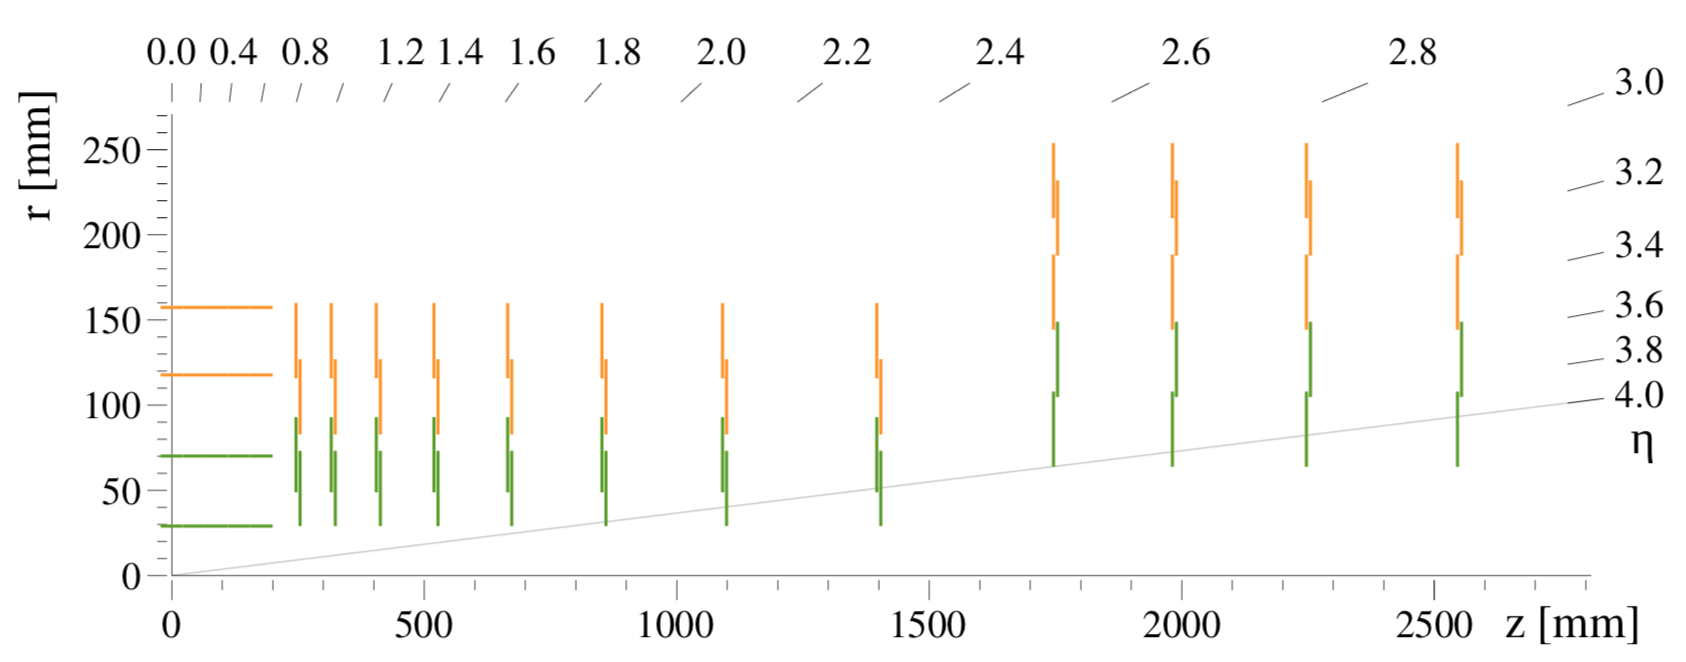
\includegraphics[width=0.63\textwidth]{figs/phase2_inner_tracker_geometry_lowres.png}
\centering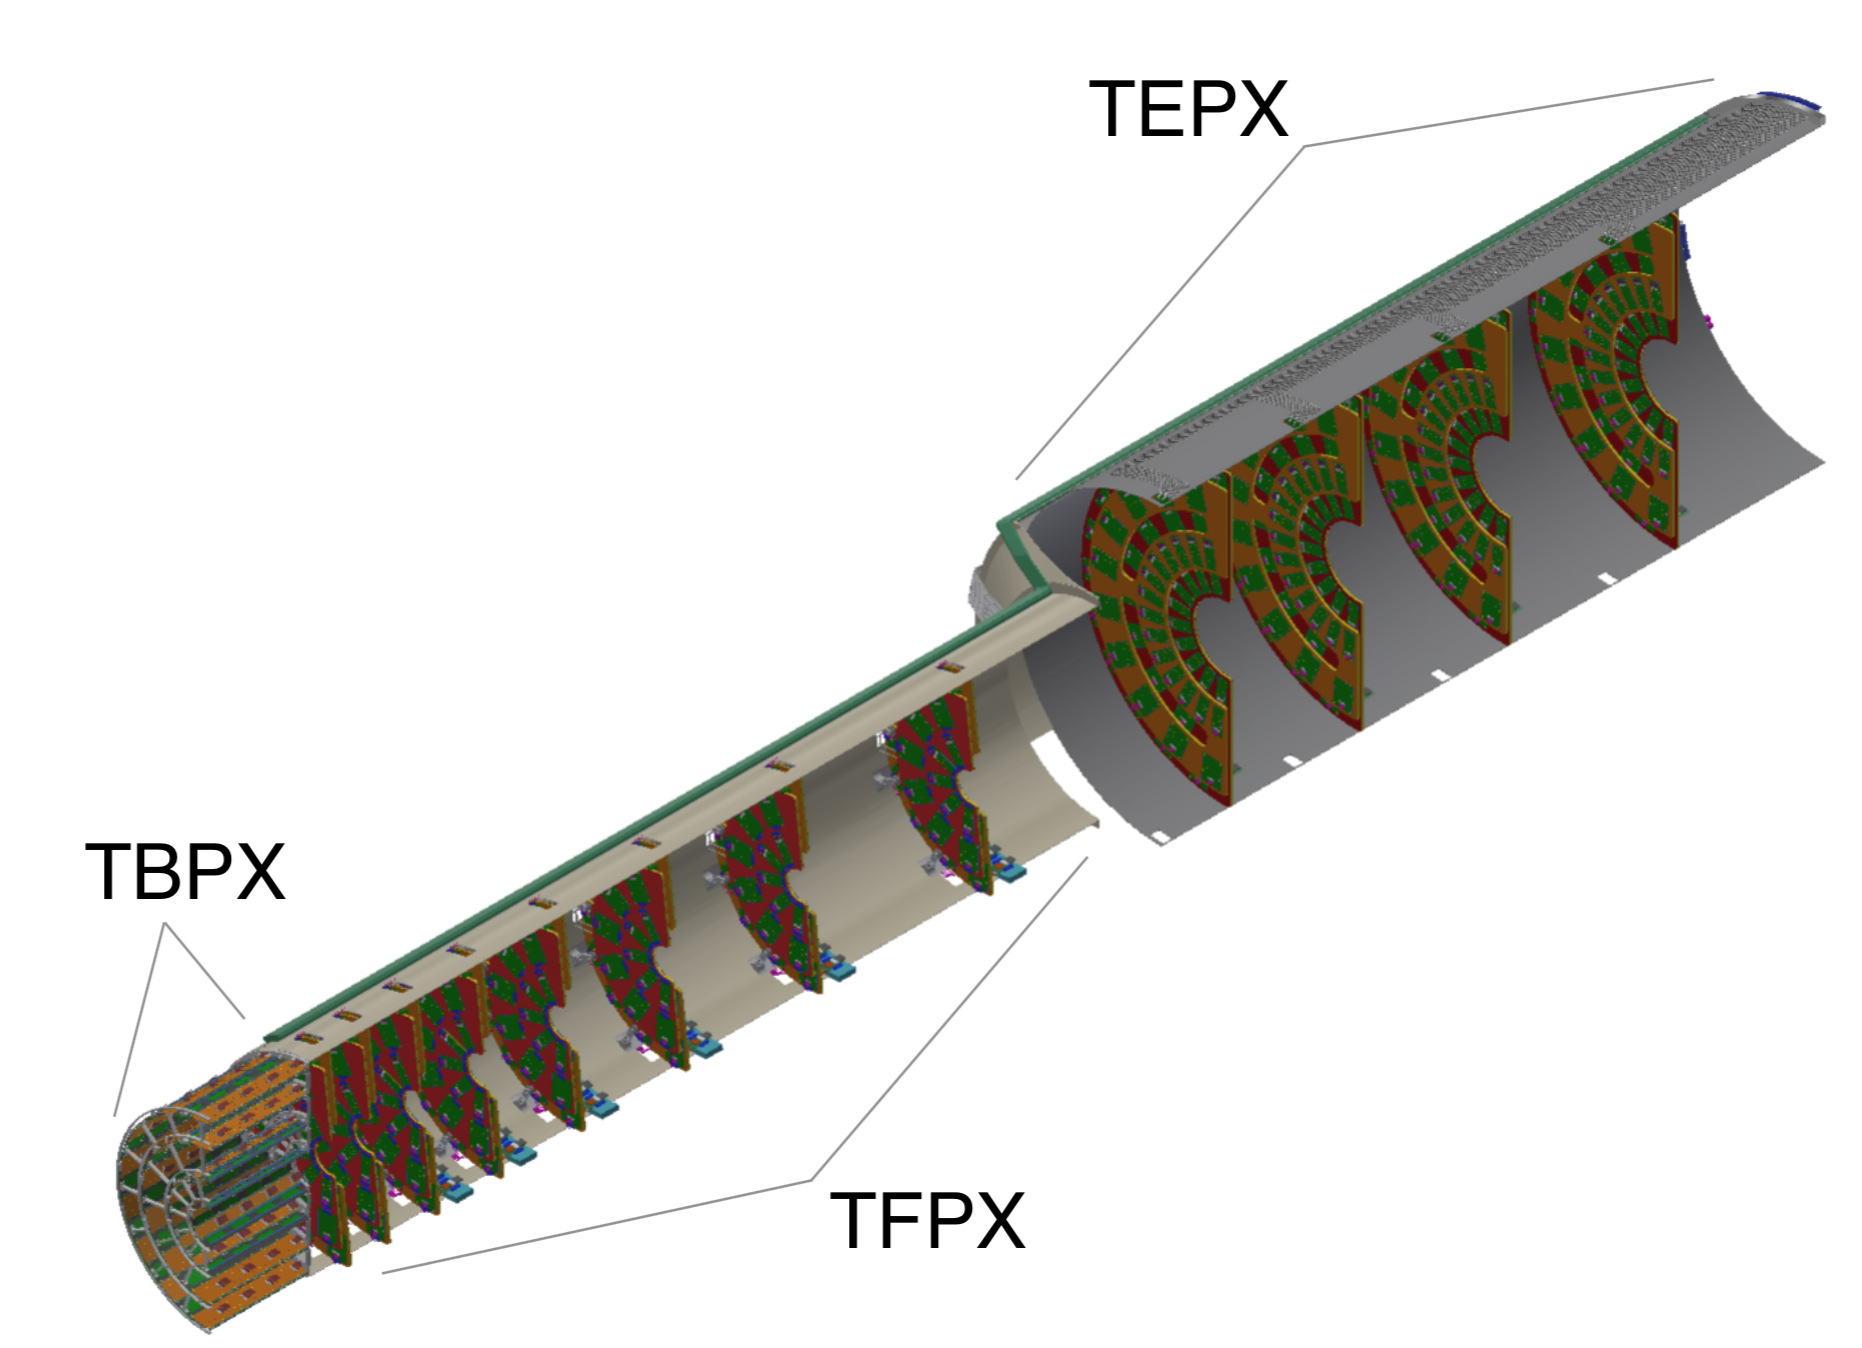
\includegraphics[width=0.35\textwidth]{figs/phsae2_inner_tracker_3D.png}
\caption{\label{fig:TFPX} Left: Geometry of the Phase-2 CMS Inner Tracker shown in $Rz$ porjection. Right: A 3D drawing of the Inner Tracker with the major subdivisions indicated.}
\end{figure}

The UNL HEP group will be produced modules for the Inner Tracker. US CMS Phase-2 upgrade project plans for three module production sites in the US for the TFPX subdetector (see Fig.~\ref{fig:TFPX}): at UNL, Purdue University, and CUA. The work on setting up the UNL site has started last summer. During the period covered by this proposal we will prepare and equip our site for TFPX module production while participating in the ongoing R\&D of the module design. Subsequently, we will run the preproduction and start on production all within these three years. The details of these activities are discussed below.

\paragraph{Production scheme and UNL site preparation}

US CMS upgrade management plans for UNL to produce about 900 modules for TFPX. Each module has three major components (see Fig.~\ref{fig:TFPXmodule}): the silicon sensor layer, the layer with several readout chips RD53A superimposed over the pixels of the sensor which has 25x100~$\mu$m granularity, and the high density interconnect (HDI). Additional components for mechanical support, such as spacers, are possible. Each production site is expected to receive "bare modules" of sensors bump-bonded to the chips by a commercial contractor as well as HDIs and other parts. The module production procedure, perfected at UNL during the production of the Phase-1 Pixel Detector several years ago, remains the same and comprises three main stages: a) gluing affixes HDIs to the bare modules in an automated procedure that uses computer-driven robotic gantry; b) wirebonding makes 400-800 electrical connections per module and is done using a high-end automatic wirebonding machine; c) wirebonds are encapsulated with a silicone elastomer using, again, the robotic gantry. Other steps of the production procedure include gluing of spacers, curing of the encapsulant in an oven, visual, electric, and mechanical quality control at different production stages, and final module quality-tier assessment. 

%XXX Add another figure here, e.g. a photo of some module prototype or RD53 drawing
\begin{figure}
\centering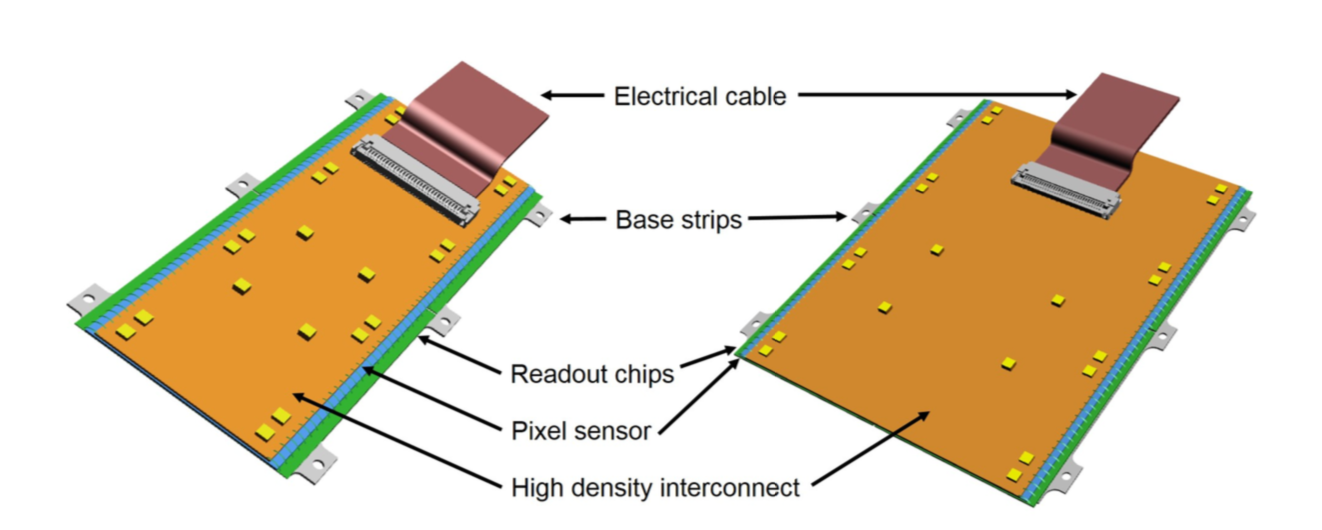
\includegraphics[width=0.45\textwidth]{figs/phase2_pixel_module_lowres.png}
%\centering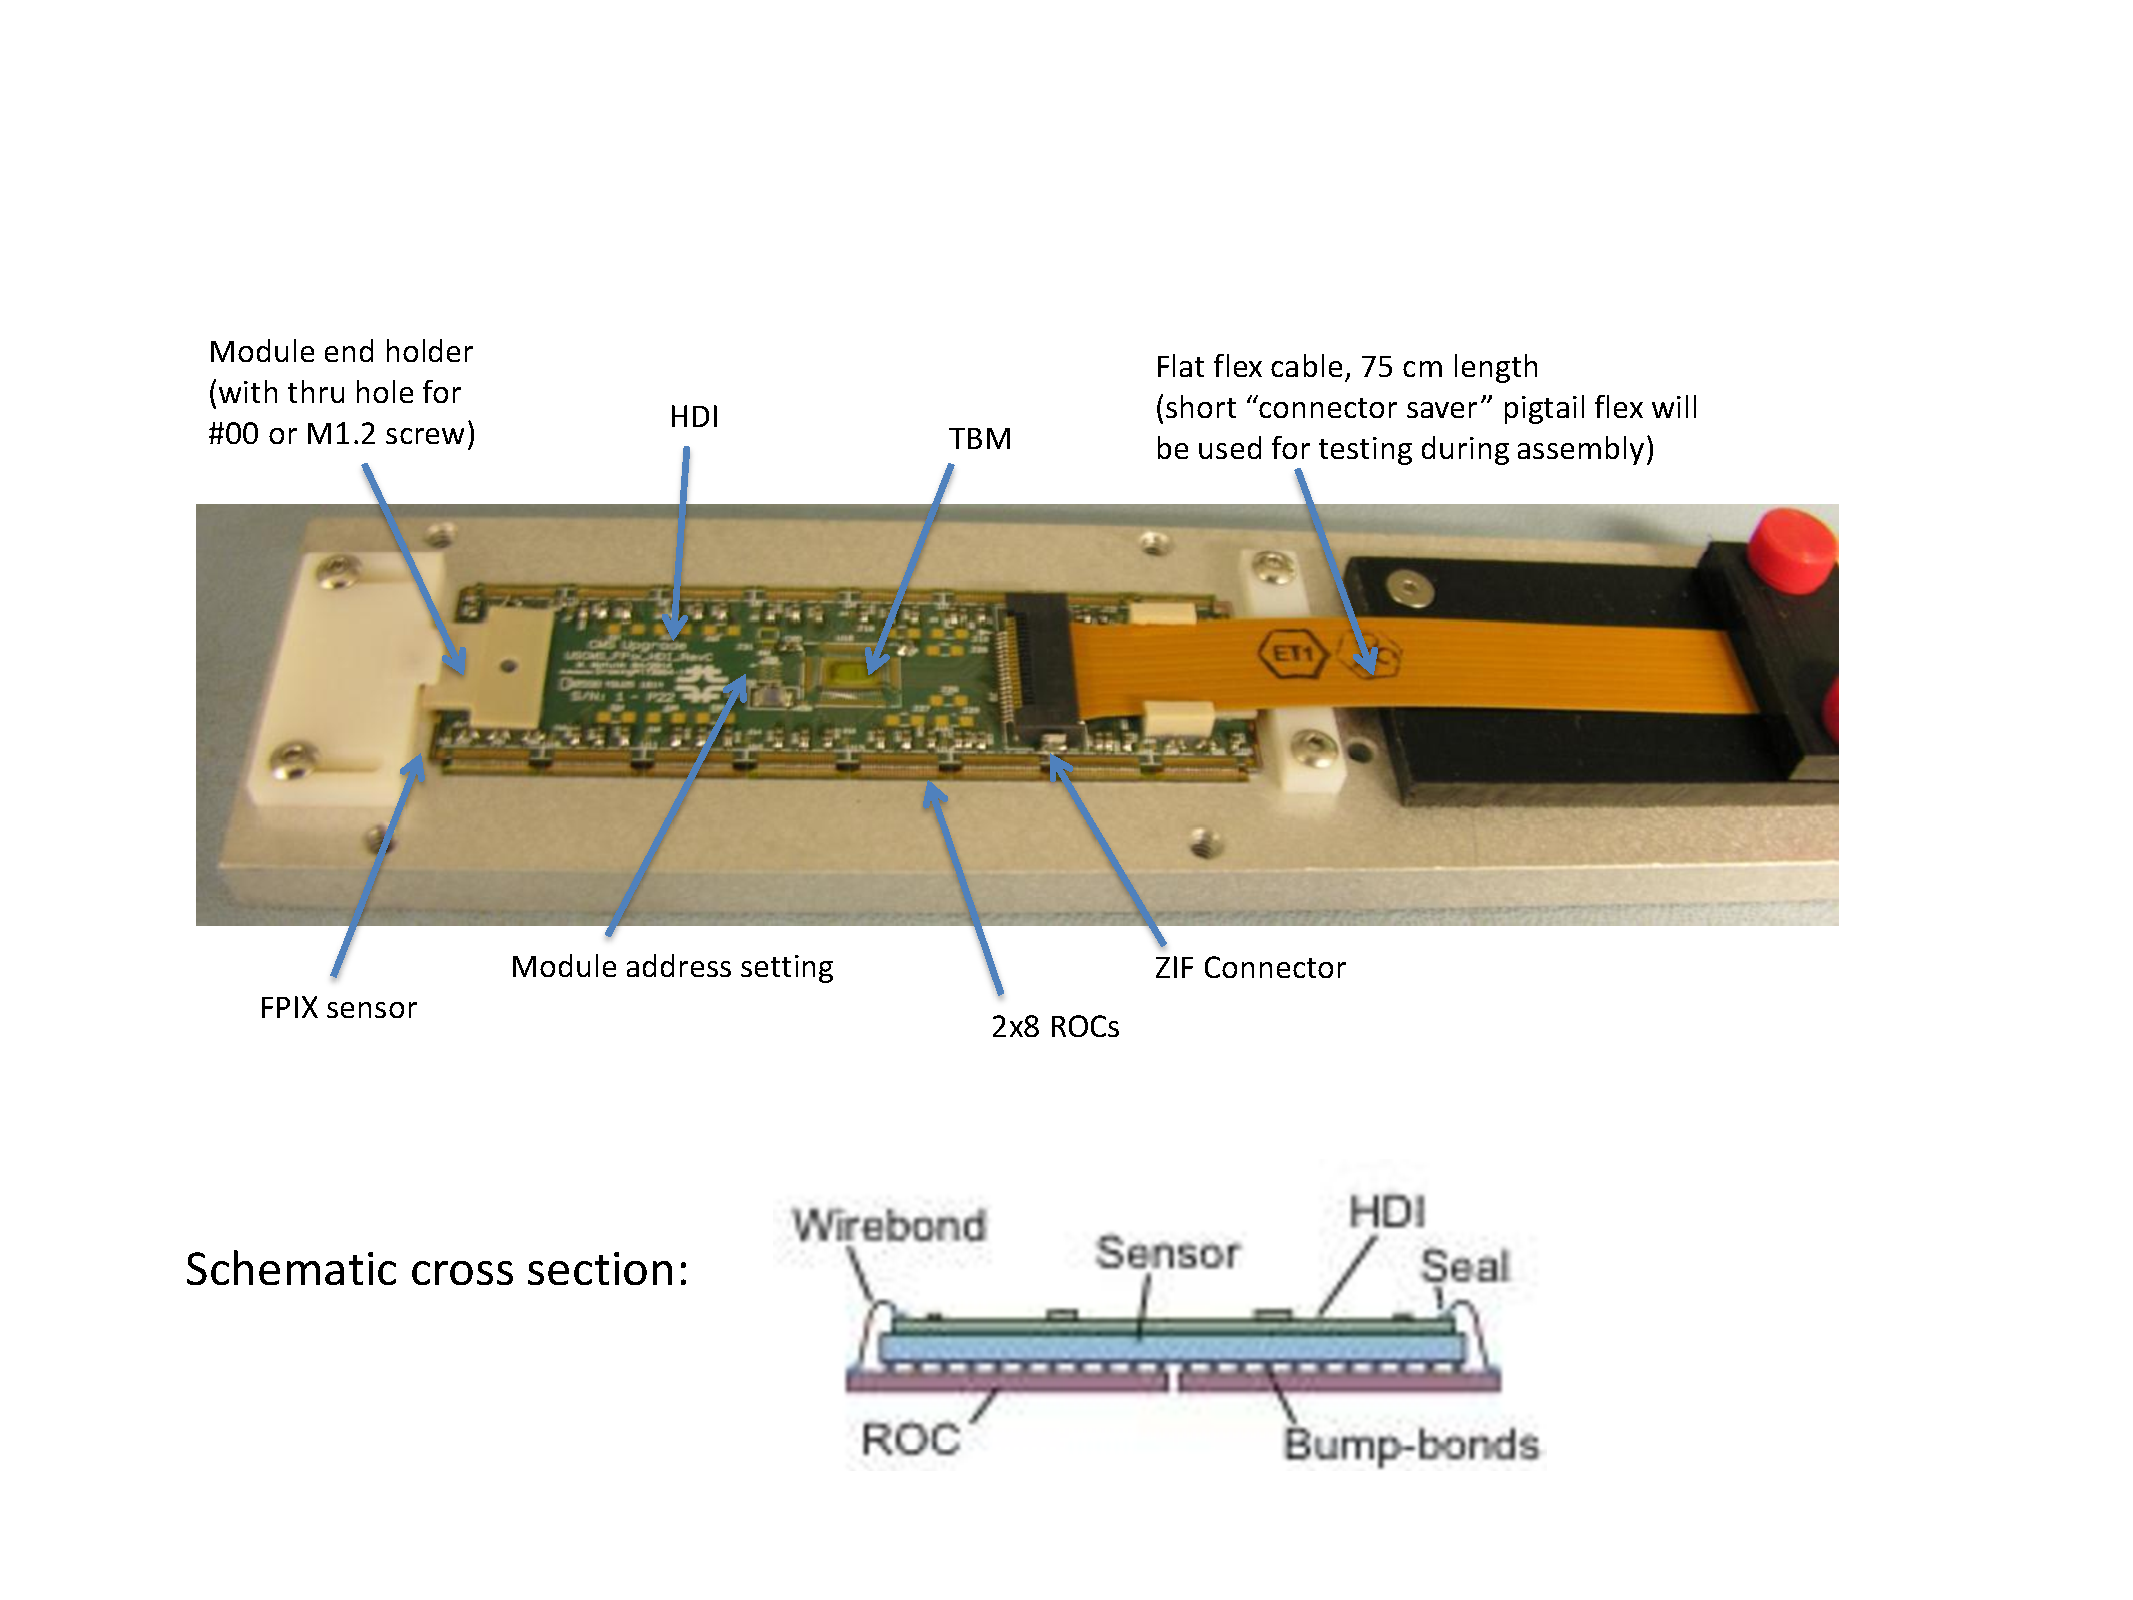
\includegraphics[width=0.45\textwidth]{figs/module}
\caption{\label{fig:TFPXmodule} Left: Conceptual view of a TFPX module with 1x2 and 2x2 readout chip layout. Right: TBA.}
\end{figure}

All of the above steps of production were working perfectly at UNL several years ago. Now, several years later, changes ocurred in personnel and equipment available. The former UNL production site, as agreed with US CMS upgrade project management, is split into two sites: UNL and CUA, with both expected to be handle equal volume of module production. Former UNL faculty member Dominguez is now a Dean of the School of Arts and Sciences and is responsible for the production center there. The key pieces of equipment, mostly funded by NSF, are split: the best wirebonder, F\&K Delvotec G5 64000, is now at UNL. The robotic gantry is at CUA. Both of our sites are expected to restore the production capacities. 

At UNL, Kravchenko, along with a postdoc and the graduate students stationed at UNL, will be running this project. Claes and Snow will contribute to some of the tasks. Presently we are recommissioning the wirebonder, recovering the skills of programming it for complex bonding patterns, and also reestablishing the clean room operation, all of this will be completed by the start of this proposal. The robotic gantry, critical to production, will have to be purchased and set up. The funds for the gantry and related equipment are in the budget of the CMS upgrade project and are outside of this proposal's budget. The gantry setup is rather complex. While the gantry can move and position its head with the accuracy of 10 microns or better, it comes "bare": custom tools need to be designed and manufactured because they are production process-specific. The examples of the tools we anticipate: pick-up tools to grab objects (vacuum-operated and mechanical), vacuum chucks to hold modules and their components, glue stamps, custom weights, glue syringe with vacuum control, positioning video cameras, and others. These will be developed in collaboration with the UNL Physics Instrument Shop, and produced in the Shop, as they have been for the Phase-1 production gantry. The software for automatic control software will be written to fit the new equipment. The baseline design at present is to use Labview running on a PC that a) controls directly movements of the gantry, b) controls vacuum lines, c) does positioning and fiducial calibration with video cameras. Additionally, the setup will include a vacuum manifold that supplues vacuum for various gantry tools and chucks controlled through by the software through a voltage controller (planned a compactDAQ from National Instruments). Several other stations will need to be set up. The visual and mechanical test station, with a microscope and wirebonding pull test capability, will need to be set up (not funded by this proposal) and will require some minor automation. The electric/digital test station will use testboards and coldbox equipment provided by FNAL and UIC, and will also need
to be set up in our lab, connected to chillers, etc, and automated as needed. These are the larger items in the list of preparing the lab equipment for production, many smaller ones are skipped due to page limit of this proposal.

\paragraph{TFPX module R\&D and beamtests}
While preparing for module production and setting up the equipment, we will continue the engagement in R\&D on module design and properties, as well as the overall Inner Detector design. Already now we are part of this work. During preparaton of this proposal, our group is participating in thermal behavior studies of the planned TFPX modules alongside with Cornell and Purdue Universities. We have wirebonded a set of "thermal mockup modules" which are designed to have the same power dissipation properties as the planned full modules, and they will be used in coldbox tests and mockup-disks at our partners' sites. We are currently working on wirebonding the most realistic to date modules that include real RD53A chips in preparation for beam tests at FNAL where the focus will be assessment of radiation resistance of the future modules. Claes and the graduate student Joaquin Siado have been involved in beam tests of TFPX prototypes at FNAL, with Siado traveling there for that purpose. Claes and Siado plan to continue this work until the chip and module design is fully settled by 2021. The modules manufactured at production sites, such as ours, will have to be thoroughly tested before they are installed in the detector. UIC will lead the development of test stands and the post-production test procedure. While we expect the most comprehensive tests to be done at UIC, before we ship our modules there we will perform a "lite-test" at UNL, using the UIC and FNAL-provided test setup. The procedure and the test setup is expected to be developed at FNAL and UIC in the period Sep 2019 to Feb 2020. It is vital that production sites participate in this development to understand the equipment, gain expertise with the chips, and make sure realistic choices are made for what constitutes the lite-test at the production site. Claes and Siado, along with the UNL postdoc with the TFPX focus, will be part of this activity. It is expected that either Siado or the postdoc will spend several month at FNAL and UIC in the beginning of the period of this proposal. Extra travel support will be requested from the CMS upgrade project or LPC visitors program for this purpose.

\paragraph{Module preproduction and production}

Module preproduction is expected to last 5-6 months during which our site will have to demonstrate its readiness. While a relatively small number of modules will be produced, this will be an intense period of making the production process seemless, running through the process of production itself and interacting with the partners upstream (from where components come) and downstream (where modules go for testing), and learning how to quickly solve production problems. Kravchenko will coordinate the preproduction and the postdoc will contribute a major effort, up to 80\% of his or her time during this period. The production period will follow. It is exepcted to last 1.5 years, with the first half a year falling under the period of this proposal. The production work will be distributed in a balanced way among the personnel including Kravchenko and Claes on the coordinating side, the postdoc, graduate and undergraduate students, and technicians from the Electronics and Instrument Shops, following the example of a successful arrangement of the Phase-1 module production at UNL.

\paragraph{Timeline and personnel}

The work described in this proposal requires significant personnel effort. Kravchenko will lead the overall TFPX effort at UNL, with Claes taking charge of several R\&D subprojects. A postdoc will be stationed at UNL and will have major responsibility in the preparation of production. The postdoc will be responsible for making sure that all stations of the production setup are ready on schedule, for setting up custom gantry tooling with the UNL Intrument Shop, and becoming expert in wirebonding by the time the production starts. Subsequently, the postdoc will have to see to preproduction successfully completing, all issues resolved, and production starting. Two or three graduate students are expected to be responsible for writing most of the software for gantry control and control of other equipment that requires it, as well as for maintaining it through the production phase. Two of the current graduate students have been major participants in the Phase-1 production software development here, and will continue helping the project and will pass their expertise to the new generation when they graduate. This project is an excellent opportunity for undergraduate researchers to get involved. During the Phase-1 production, a number of undergraduates executed simpler projects of site preparation and for Phase-2 we expect to continue this tradition. The first planned projects for undergraduates include, for example, automatic control of an oven for curing encapsulated wirebonds with a simple electronics board with, e.g., an Arduino chip that switches power supply on and off, and a thermocouple, or video camera control for taking diagnostic photos of the modules at different production stages. Finally, the wirebonding operation will be, to a significant degree, done by the UNL Electronics Shop technicians who participated in the Phase-1 production as well (their time is in the budget of the CMS upgrade project and not in this proposal).

The timeline of this project is driven by the schedule of the Us CMS Phase-2 upgrade as well the time when NSF plans to fund major equipment acquisition. The milestones are listed in the table below.

\vspace{3mm}
\noindent
\begin{tabular}{l|l}
\hline
present - Apr 2020 & clean room recommissioning, some equipment setup, wirebonding operations \\
        &  R\&D and testbeam participation \\
Apr 2020 - May 2021 
         & major equipment (gantry, etc) is provided by the project \\
         & gantry custom tooling, software development, finish production preparation \\
Jun 2021 - Nov 2021
         & TFPX module preproduction, address any issues that arise \\
Dec 2021 - Jul 2023 
         &  TFPX module production (900 modules planned) \\
\hline
\end{tabular}

\subsection{CMS Detector Operations}
An experimental apparatus as complex as the CMS Detector requires a large crew of experts taking care of it 24/7 online and offline. The experiment has a team of shifters responsible for the central detector systems, the Shift Leader for the team, and several Run Field Managers who oversee multiple shift crews over longer time periods. Additionally, each subdetector has dedicated experts on call. All CMS signing authors are expected to participate in the activities of data taking. The UNL HEP group goes beyond simple shift duties: members of the group stationed at CERN will contribute at key points of detector operations.  Our postdocs and sometimes even graduate students routinely serve in position of a Run Field Manager, a position near the top of data taking coordination hierarchy, in a position of a Shilft Leader, and as experts-on-call for the CMS pixel detector operation. All UNL HEP graduate students stationed at CERN will be expected to take the most critical central shifts, managing the Data Acquisition, Trigger, and Data Quality Monitor systems. While the operations during the calendar year 2019 and the first half of 2020 are expected to be on the light side, experts at CERN, such as our group members, will still be needed to keep parts of the detector running running the experiment in the cosmic rays detection mode. In the second half of 2020 we expect rapid ramp-up and recommissioning of the detector and intense activities from the beginning of 2021 and on as Run-3 commences. 
